\newcommand{\versionnumber}{1.0}
\newcommand{\docversion}{
  \renewcommand{\arraystretch}{0.5}
  \setlength{\tabcolsep}{0pt}
  \begin{tabular}[b]{l}
  Versie \versionnumber{}\\
  \today \\
  \end{tabular}
}
\newcommand{\doctitle}{KBS ESA3 \\ Functioneel Ontwerp \\ Smart Markers}
\newcommand{\doctitleshort}{FO - Smart Markers}
\newcommand{\docauthor}{
  \renewcommand{\arraystretch}{0.5}
  \begin{tabular}{l l}
  Jerko Lenstra & {\mdseries(S1080179)} \\
  Rick de Bondt & {\mdseries(S1078239)} \\
  Marthijn Tijmes & {\mdseries(S1063534)} \\
  \end{tabular}
}

\newcommand{\doctitlepage}{
  \thispagestyle{empty}

  \parbox[t]{1.0\linewidth}{
    \fontsize{40pt}{60pt}\selectfont
    \doctitle{}
    \fontsize{20pt}{40pt}\selectfont
    \\hbo-ICT, Windesheim
    \\Docent: Gido Hakvoort
  }

  \setlength{\wpYoffset}{-1.8cm}
  \ThisCenterWallPaper{0.75}{functional/windesheim_kadaster.png}
  \vfill

  {
   \docversion{}
   \hspace{185pt}
   \docauthor{}
  }

  \normalcolor{}

  \newpage
}

\providecommand{\doctitle}{Title}
\providecommand{\docauthor}{Author}
\providecommand{\doctype}{scrartcl}
\providecommand{\doctitlepage}{TitlePage}

\documentclass[12pt,a4paper,titlepage,parskip=half]{\doctype}

\usepackage[dutch]{babel}
\usepackage{blindtext}
\usepackage{float}
\usepackage[hidelinks]{hyperref}
\usepackage{graphicx}
\usepackage{listings}
\usepackage{wallpaper}
\usepackage[headsepline,footsepline,manualmark]{scrlayer-scrpage}


% Input and output encoding ---------------------------------------------------
\usepackage{iftex}
\ifPDFTeX
   \usepackage[utf8]{inputenc}
   \usepackage[T1]{fontenc}
   \usepackage{lmodern}
\else
   \ifXeTeX
     \usepackage{xltxtra}
   \else
     \usepackage{luatextra}
   \fi
   \defaultfontfeatures{Ligatures=TeX}
\fi

% Math
\usepackage{amsmath}
\usepackage{amsfonts}
\usepackage{amsthm}
\usepackage{amssymb}
\usepackage{mathtools}

\DeclarePairedDelimiter{\ceil}{\lceil}{\rceil}
\DeclarePairedDelimiter{\floor}{\lfloor}{\rfloor}
\DeclarePairedDelimiter{\bag}{\langle}{\rangle}
\DeclarePairedDelimiter{\set}{\{}{\}}

% Misc
\usepackage[shortlabels]{enumitem}
\usepackage{pgfgantt}

% Bibliography
\usepackage{csquotes}
\usepackage[natbib,style=apa,citestyle=authoryear]{biblatex}
\DeclareLanguageMapping{dutch}{dutch-apa}
\defbibheading{bibliography}[\bibname]{\section{#1}}
\addbibresource{functional/bibliography.bib}

% Display
\usepackage{lastpage}
\usepackage{tabularx}
\usepackage{eurosym}
\setlength{\headheight}{24pt}

\title{\doctitle}
\author{\docauthor}
\date{\today}

\ihead{\upshape{\doctitleshort}}
\ohead{\upshape{\today, v\versionnumber}}
\cfoot{\upshape{\thepage\ /~\pageref{LastPage}}}

\numberwithin{equation}{section}
\numberwithin{figure}{section}
\numberwithin{table}{section}

\usepackage{changepage}

\usepackage{enumitem}
\setitemize{noitemsep,topsep=0pt,parsep=0pt,partopsep=0pt}

%Other settings
\lstset{basicstyle=\ttfamily}

\RedeclareSectionCommand[beforeskip=1\baselineskip,
                         afterskip=.25\baselineskip]{section}

\RedeclareSectionCommand[beforeskip=.25\baselineskip,
                         afterskip=.25\baselineskip]{subsection}

\RedeclareSectionCommand[beforeskip=.25\baselineskip,
                         afterskip=.25\baselineskip]{subsubsection}

\RedeclareSectionCommand[beforeskip=.25\baselineskip,
                         afterskip=.25\baselineskip]{paragraph}


\begin{document}
\doctitlepage{}

\tableofcontents
\thispagestyle{empty}
\newpage

\clearpage
\setcounter{page}{1}
\addtocontents{toc}{\protect\thispagestyle{empty}}

\newpage
\section{Documenthistorie}

\begin{tabularx}{\textwidth}{| l | l | X | l |}
    \hline
    \textbf{Versie} & \textbf{Datum} & \textbf{Verandering} & \textbf{Auteur(s)} \\ \hline
    0.1 & 20-nov-2017 & Aanmaken document & Rick de Bondt \\ \hline
    0.2 & 21-nov-2017 & Invullen document & Rick de Bondt \\ \hline
    1.0 & 27-nov-2017 & Aanpassen milestones en spelling & Marthijn Tijmes \\ \hline
\end{tabularx}


\newpage
\section{Inleiding}
In Nederland is het vanzelfsprekend dat vastgoed geregistreerd is en dat er bekend
is welke gegevens bij dat vastgoed horen. Het Kadaster is verantwoordelijk voor de
vastlegging en verstrekking van vastgoed- en geografische informatie en de rechten
die daarbij horen, zoals eigendom en hypotheek. \citep{KAD_OVER}

Nederland is op gebied van kadastrale registratie vooruitstrevend; in het buitenland
is het niet vanzelfsprekend dat gegevens van vastgoed ergens zijn vastgelegd.
Als gevolg daarvan kan men in deze landen niet aantonen wat hun ontroerend goed is
of wat de waarde daarvan is.

Uit de morele overtuiging dat iedereen recht op eigendom heeft, wat onder andere
opgenomen is in artikel 17 van de Universele Verklaring van de Rechten van
de Mens (UVRM) \citep{UN_UDHR}, wil het Kadaster International deze landen een systeem bieden waarmee
deze eigendommen in kaart gebracht kunnen worden. Dit systeem is recentelijk in
ontwikkeling genomen en het project draagt de naam: \textit{Smart Markers}

\subsection{Aanleiding}
Door het Internet-of-Things keuzesemester van de opleiding hbo-ICT, te Windesheim,
zijn de uitvoerende studenten in aanraking gekomen met dit project. Tijdens het
keuzesemester is er een periode van tien weken waarin studenten aan een project
werken wat in het kader staat van (inter)connectiviteit, duurzaamheid en in het
belang is van de maatschappij.

\subsection{Doel}
Het doel van het project is om ontwikkelingslanden een systeem te bieden dat
een soortgelijke werking heeft als de kadastrale registratie van het Kadaster
in Nederland.

Binnen de scope van tien weken betekent dit het ontwikkelen van een prototype
van een systeem waar locatiegegevens mee kunnen worden verzameld. In hoofdstuk
\ref{sec:opdracht} wordt dit systeem verder uitgediept.


\newpage
% Pad with two zeroes
\newcommand\padzeroes[1]{\ifnum #1 < 10 0\fi\ifnum #1 < 100 0\fi #1}

% This stuff does automatic user story numbering
\newcommand{\ustorylbl}{FREQ}
\newcounter{storynr}
\newcommand{\story}{\subsubsection{\ustorylbl-\padzeroes{\arabic{storynr}}}}
\stepcounter{storynr}

\section{Eisen}
\subsection{User Stories}
\story
Als Kadaster medewerker wil ik de locatie van de Smart Markers kunnen zien via
een kaart.
\stepcounter{storynr}

\story
Als Kadaster medewerker wil ik de Smart Markers kunnen identificeren.
\stepcounter{storynr}

\story
Als Kadaster medewerker wil ik kadastrale registratie kunnen doen,
met behulp van de Smart Markers kaart.
\stepcounter{storynr}

\story
Als Smart Marker plaatser wil ik kunnen zien dat een Smart Marker aanstaat.
\stepcounter{storynr}

\story
Als Smart Marker plaatser wil ik kunnen zien dat een Smart Marker verbonden
is met het netwerk.
\stepcounter{storynr}

\story
Als Smart Marker plaatser wil ik geen systeem instellingen hoeven aan te passen.
\stepcounter{storynr}

\story
Als Smart Marker plaatser wil ik weinig onderhoud hoeven te doen aan de
Smart Marker (Batterij duur).
\stepcounter{storynr}

\newpage
\subsection{Milestones}
\begin{itemize}
    \item Een prototype van een enkele Smart Marker dat zijn locatie kan bepalen
    \item Een tweede Smart Marker dat met het eerste Smart Marker kan communiceren
    \item Vijf Smart Markers die met elkaar kunnen communiceren
    \item Een weergave van de locatie van de verschillende Smart Markers op
          een kaart
\end{itemize}
\subsection{Definition of Done}
Iets is pas klaar als:
\begin{itemize}
    \item De code geschreven is volgens de code standaard die in het plan
          van aanpak beschreven is.
    \item De code volledig is getest volgens ons testplan.
    \item De code ook unittests heeft waar het nodig is.
    \item De documentatie klopt met de code
    \item De code is gereviewd door tenminste één teamgenoot
\end{itemize}


\newpage
\section{Gebruikersinterface}

De gebruikersinterface maakt het inzichtelijk op een kaart waar de door de
SmartMarkers gemeten punten zich bevinden. Daarnaast is het mogelijk om op
deze kaart percelen aan te maken, om de meetpunten ook daadwerkelijk te
gebruiken.

\subsection*{Eerste weergave}
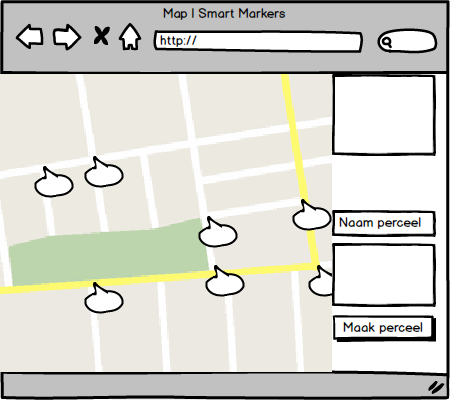
\includegraphics{functional/map_1.png}
Wanneer de wegpagina bezocht wordt, toont deze een kaart met de daarop reeds
ontvangen meetpunten uit de database.

\subsection*{Meetpunt selecteren}
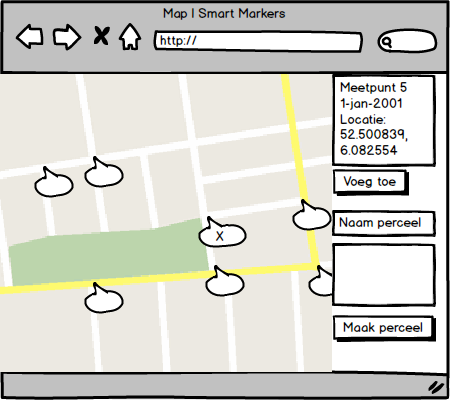
\includegraphics{functional/map_2.png}
Wanneer één van de meetpunten geselecteerd is, wordt in de informatiebox
rechtsboven de beschikbare informatie als naam, locatie en tijdstip van meten
getoond.
Daarnaast komt er een 'Voeg toe' button in beeld, welke het mogelijk
maakt om een X aantal meetpunten aan een lijst met meetpunten voor een nieuw
te maken perceel toe te voegen.

\subsection*{Perceel aanmaken}
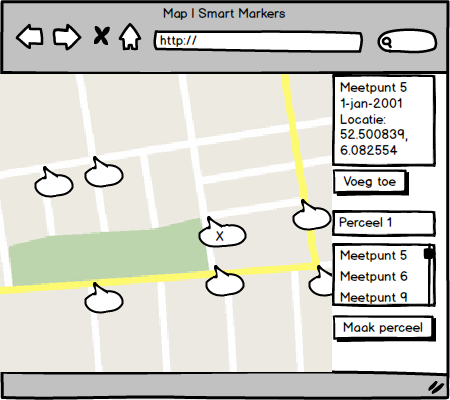
\includegraphics{functional/map_3.png}
De tekstbox met 'Naam perceel' kan gebruikt worden om een naam voor het perceel
in te geven. Daarnaast is een lijst gemaakt van toegevoegde meetpunten. Door op
de 'Maak perceel' button te klikken wordt de huidige selectie, met naam, als een
nieuw perceel op de kaart weergegeven

\subsection*{Perceel aangemaakt}
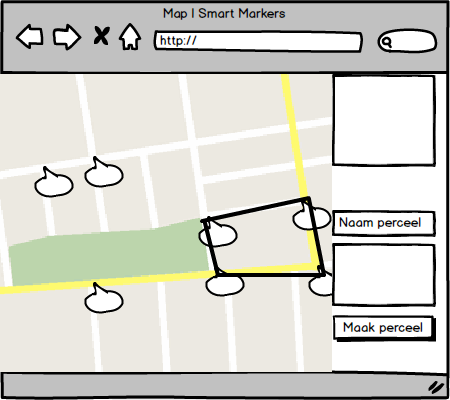
\includegraphics{functional/map_4.png}
Na het op 'Maak perceel' klikken, wordt scherm gelijk aan de eerste weergave
getoond, met het verschil dat het zojuist gemaakte perceel nu zichtbaar gemarkeerd
op de kaart getoond wordt.

\subsection*{Perceel selecteren}
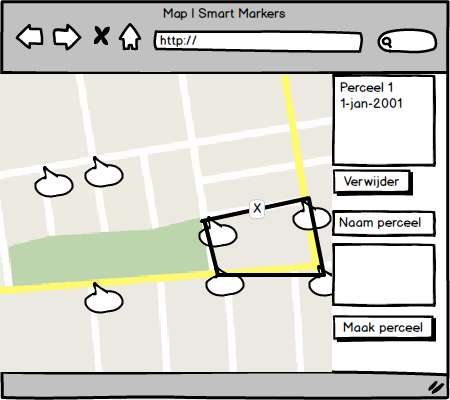
\includegraphics{functional/map_5.png}
Wanneer één van de gemaakte percelen geselecteerd is, wordt in de informatiebox
rechtsboven de naam en het tijdstip van creëren van het perceel getoond.
Daarnaast komt er een 'Verwijder' button in beeld, welke het mogelijk maakt het
geselecteerde perceel te verwijderen. Door hier op te klikken wordt dit perceel
uit de database verwijderd.


\newpage
\section{Middelen}
\subsection{Kosten}
\subsection{Teamleden}


\newpage
\section{Risico's}
\subsection{Risico Analyse}



\newpage
\printbibliography

\end{document}
